
%  \section{The analysis of FWHM behavior} 

Now that we understand (heopfully) that the seeing is by and large described by 
a single parameter, FWHM, we study three aspects of its variation, as follows.


\subsection{The FWHM dependence on wavelength} 

Asumming a power law, FWHM$\propto \lambda^{-\alpha}$, what can we say 
about $\alpha$ distribution? 

\begin{figure}
\centering
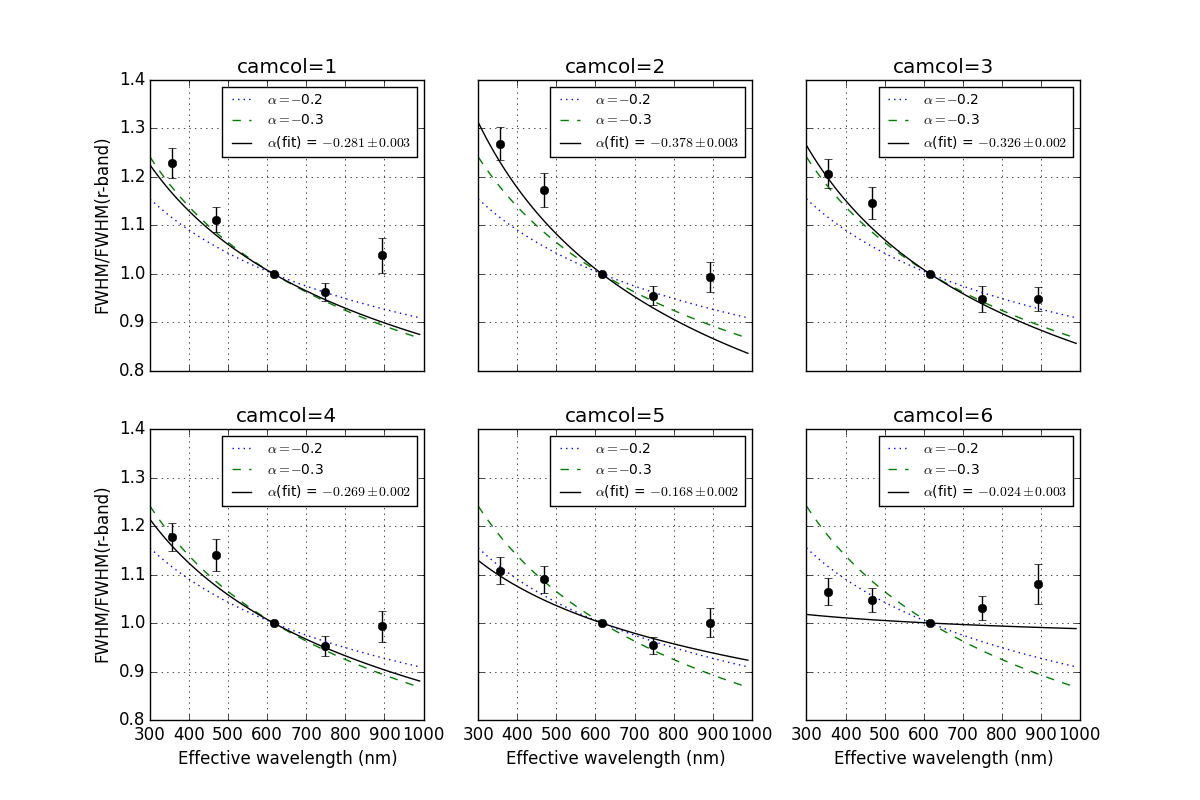
\includegraphics[width=0.9\textwidth]{FIGURES/fwhm_lambda.png}
\caption{FWHM as functions of wavelength for run 4874.
\label{fig:fwhm_lambda}}
\end{figure}



\subsection{Angular structure function} 

Cross-correlation of FWHM for 6 camera columns and the measurement of the angular
structure function (that is, the covariance vs. angular distance). 

\begin{figure}
\centering
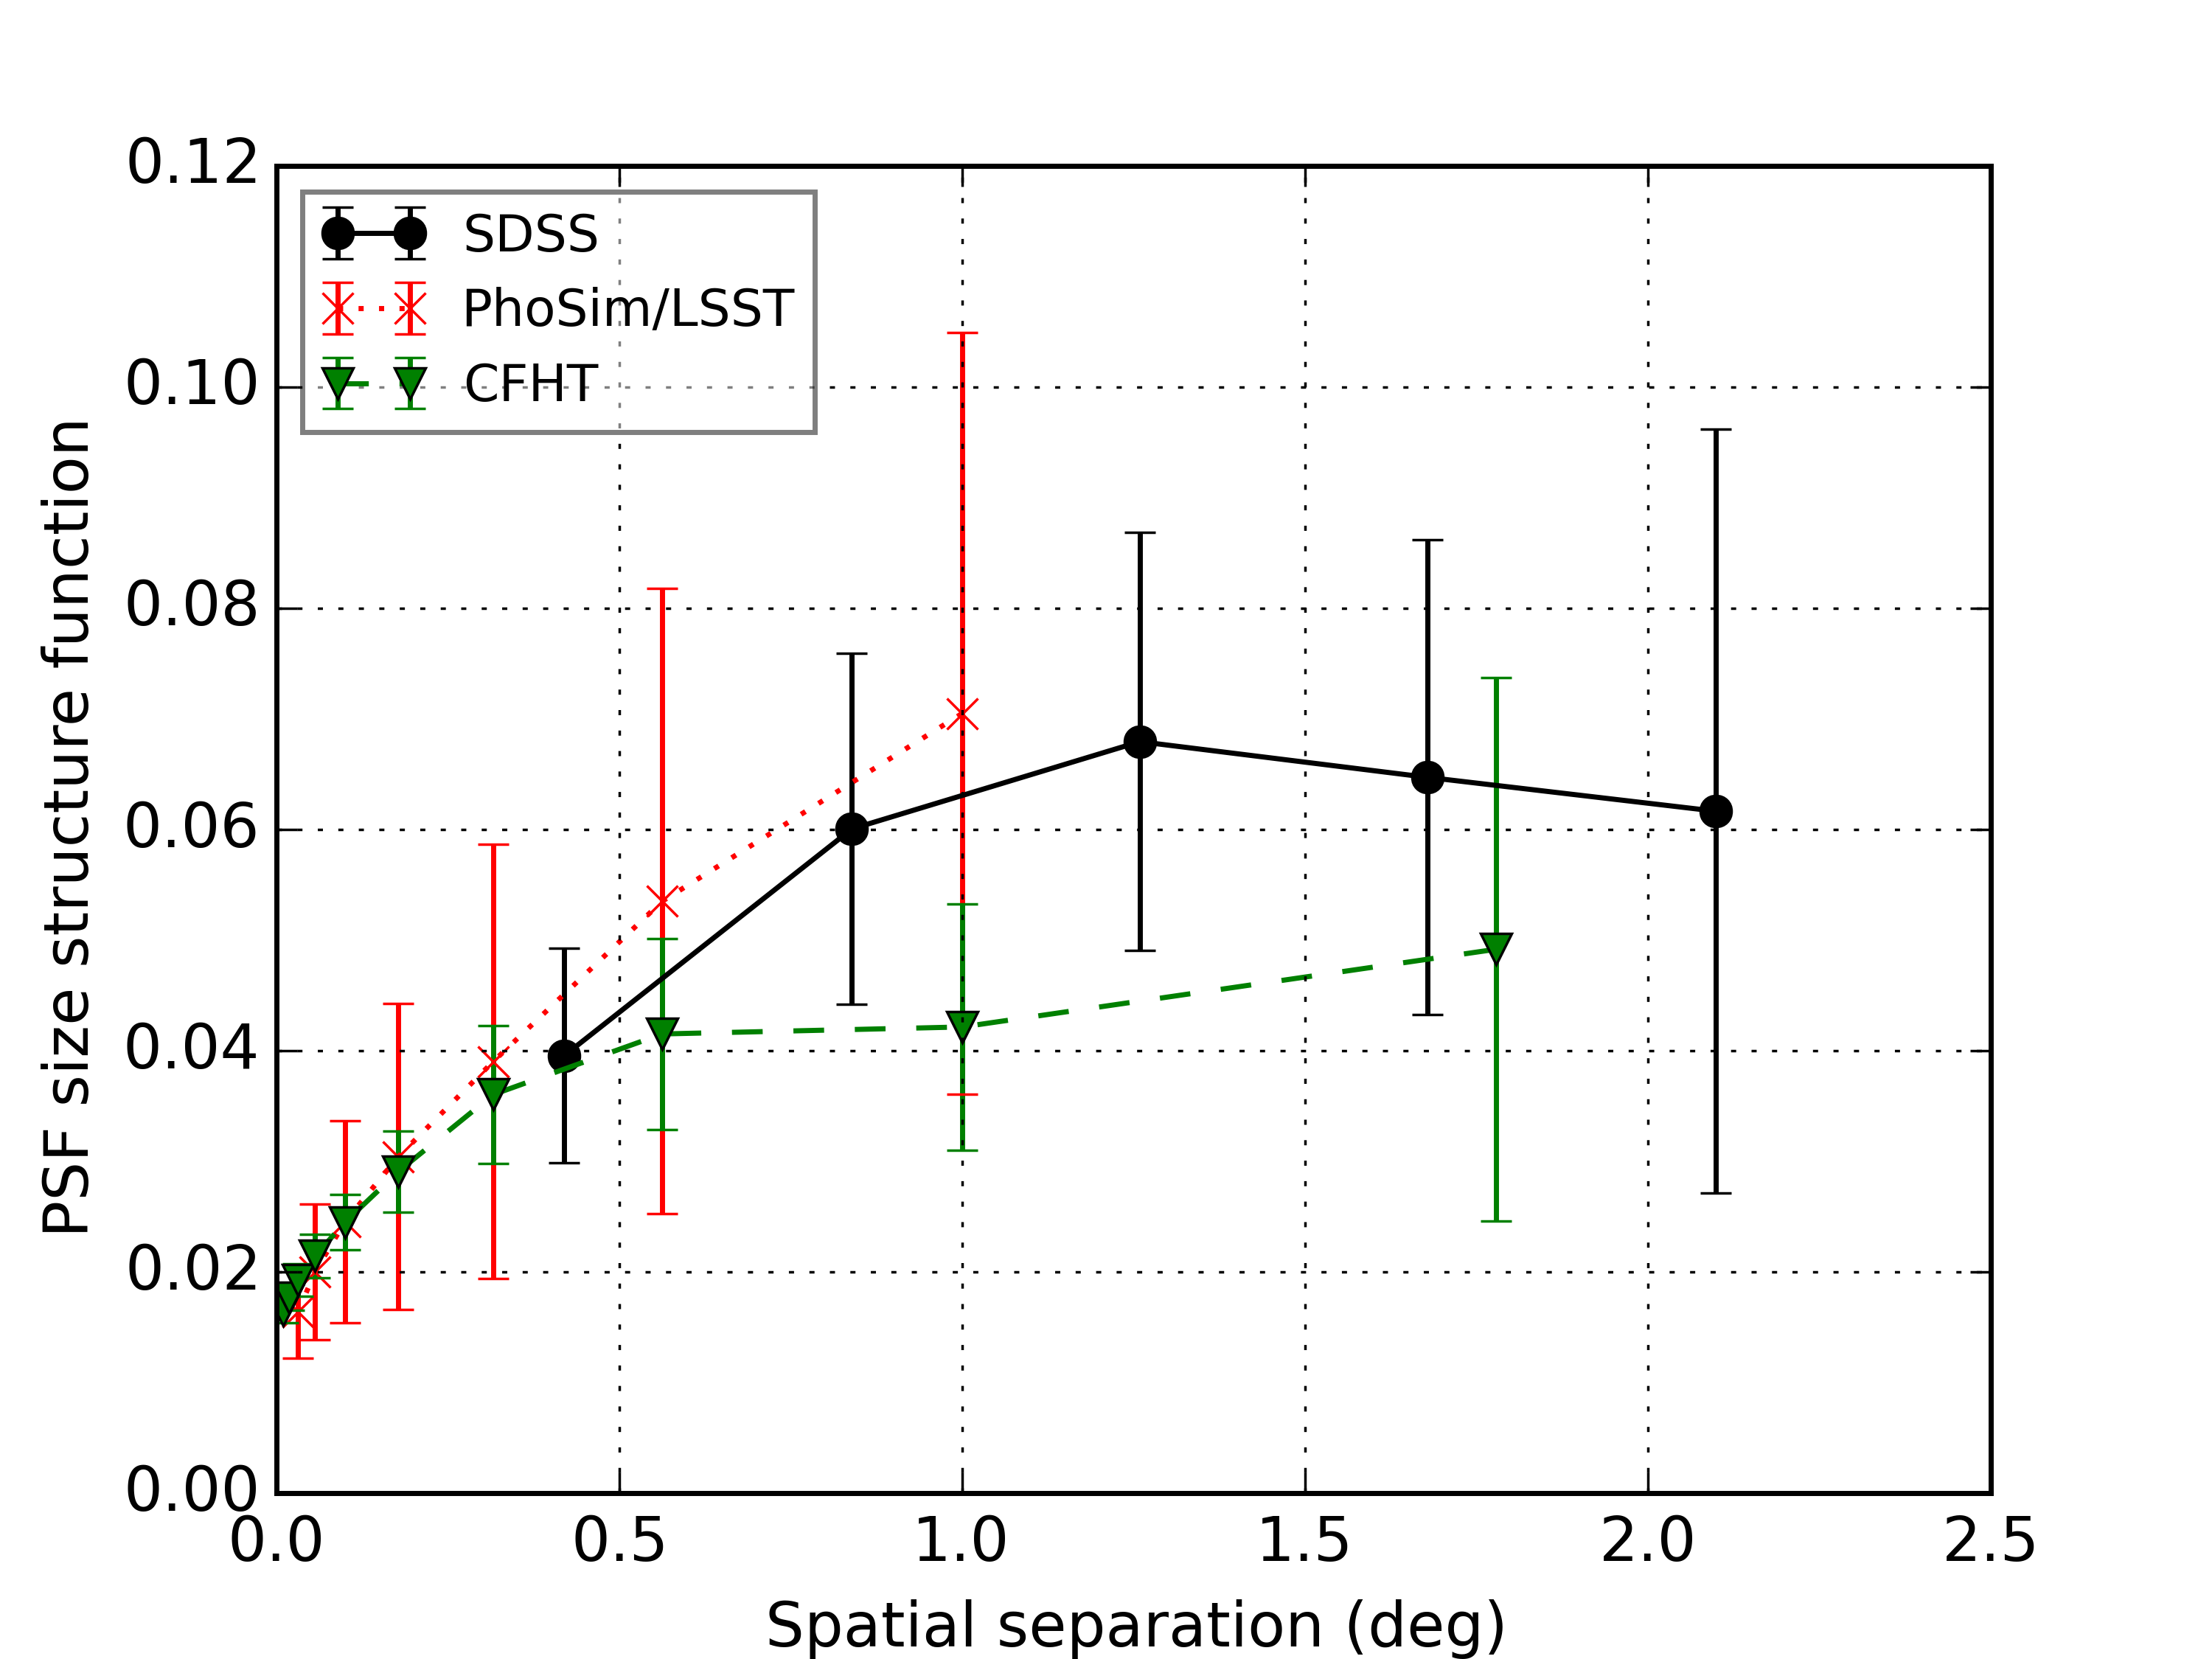
\includegraphics[width=0.9\textwidth]{FIGURES/spatial.png}
\caption{spatial correlation for run 1009. 
\label{fig:fwhm_lambda}}
\end{figure}

\subsection{Temporal auto-correlation function}

Study the temporal power spectrum:
\begin{itemize}
\item Let's start with plain Fourier transform and look at power spectra (we can 
    play games with co-addition, 6 columns for a given run, or all runs)
\item Potentially, we could also look at  Kelly and Becker code  (2014, ApJ 788, 33) 
\item Here we can compare to Chuck's CP measurements (in opsim db) 
\end{itemize} 

\begin{figure}
\centering
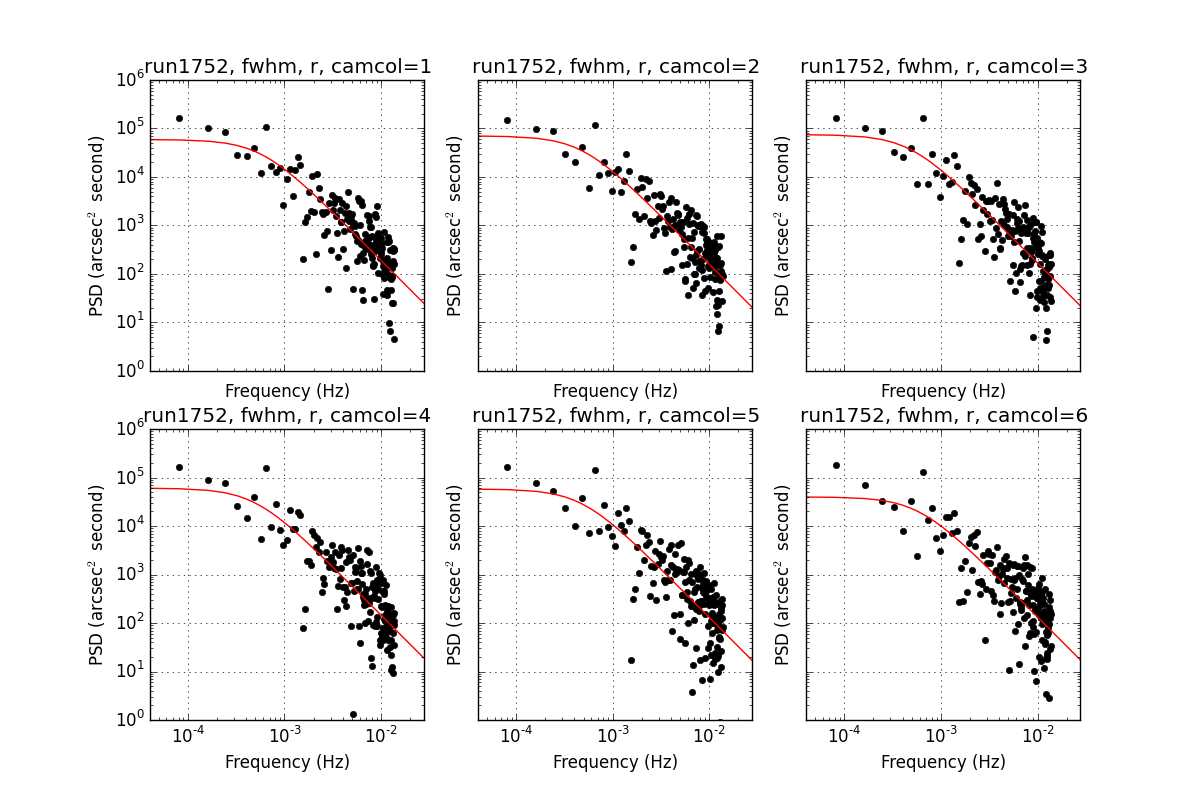
\includegraphics[width=0.9\textwidth]{FIGURES/temporal.png}
\caption{spatial correlation for run 1752. Average
  $f_0 = 5.1\times 10^{-4} Hz$, Average $\tau = 314 sec.$ 
\label{fig:psd}}
\end{figure}

\begin{figure}
\centering
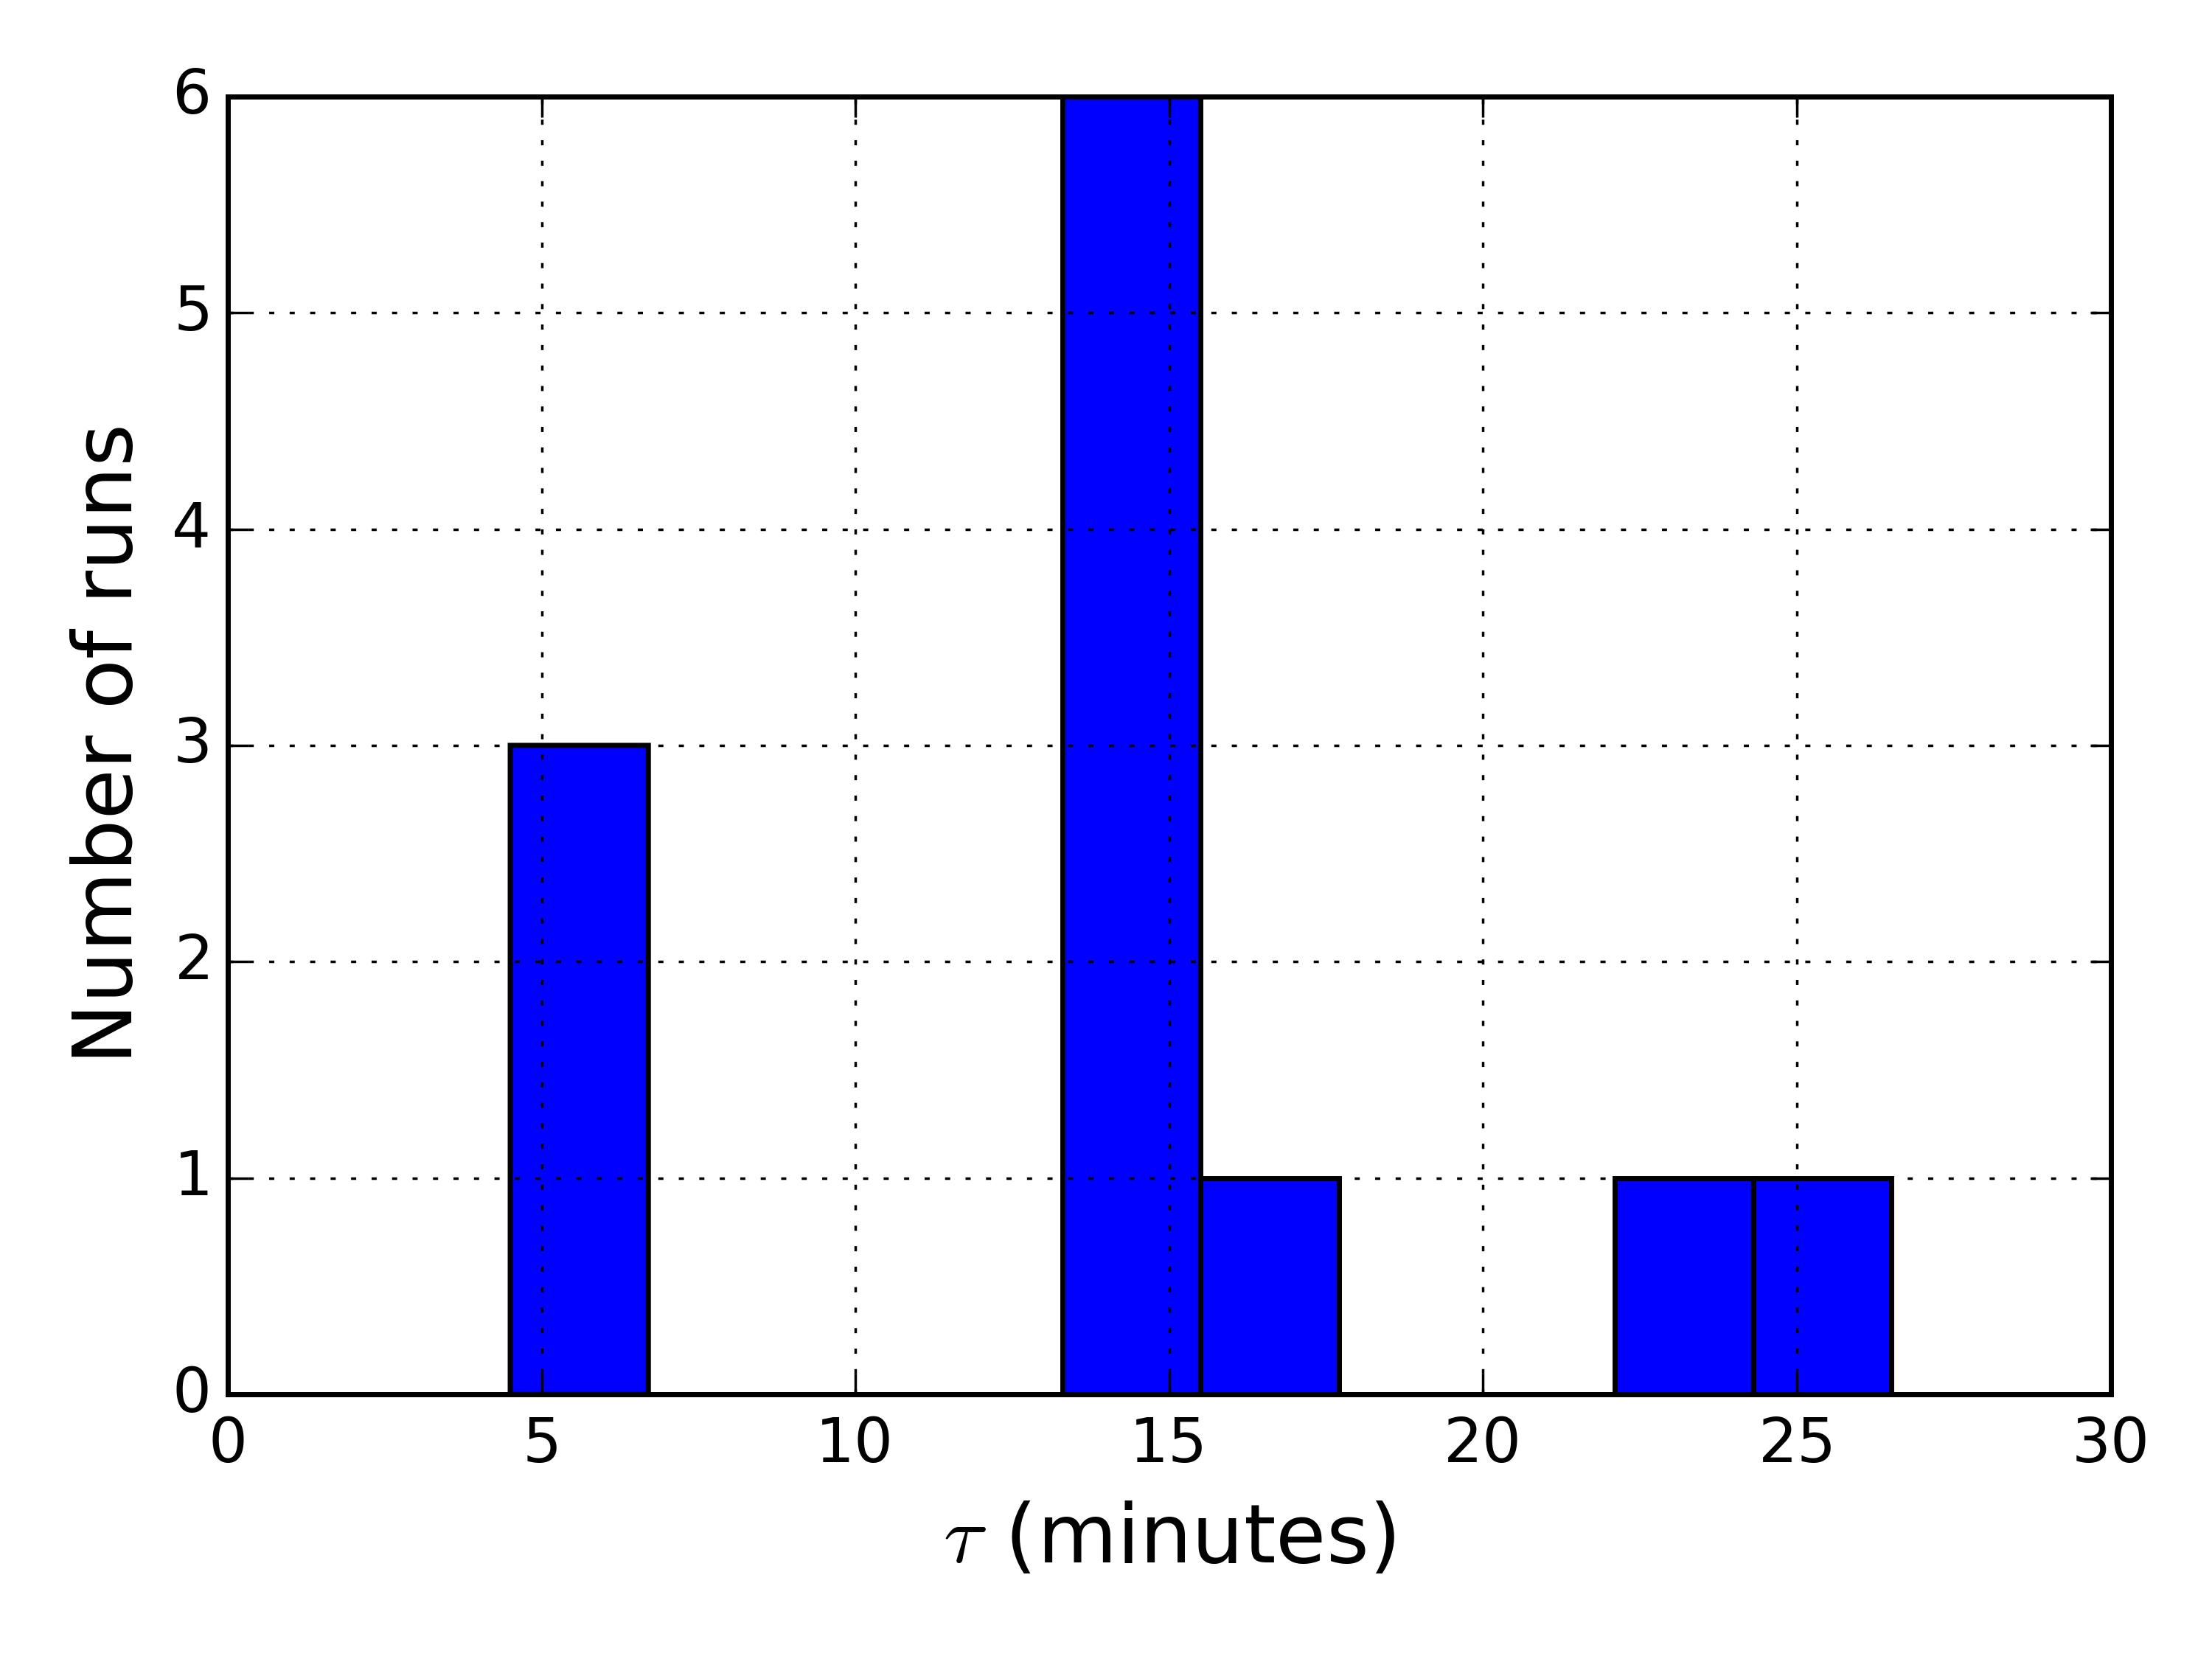
\includegraphics[width=0.9\textwidth]{FIGURES/hist.png}
\caption{histograms
\label{fig:hist}}
\end{figure}


\begin{figure}
\centering
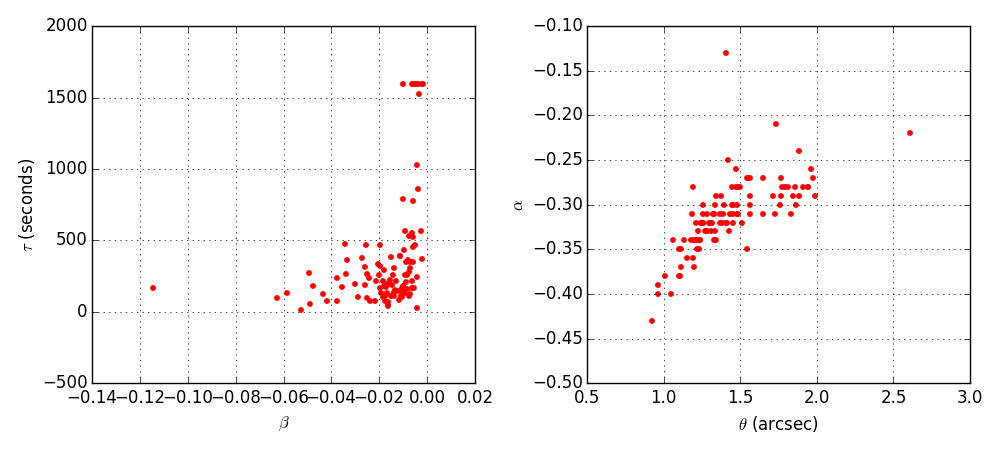
\includegraphics[width=0.9\textwidth]{FIGURES/correlate.png}
\caption{correlations  from all 108 runs.
\label{fig:correlate}}
\end{figure}



\begin{table}[t!]
\caption{A little stolen table to test if it works here... It does! }
\vskip 0.05in
\begin{tabular}{|l|c|c|c|c|c|}
\hline  
    $r$   &  $\sigma^a_{xy} $  & $\sigma^b_\pi$  &   $\sigma^c_\mu$   &  $\sigma^d_1$  &  $\sigma^e_C$  \\
    mag &       mas            &      mas  & mas/yr &   mag   &    mag  \\
\hline  
       21 &  11  &  0.6  &  0.2   &   0.01  &   0.005 \\
       22 &  15  &  0.8  &  0.3   &   0.02  &   0.005 \\
       23 &  31  &  1.3  &  0.5   &   0.04  &   0.006 \\
       24 &  74  &  2.9  &  1.0   &   0.10  &   0.009 \\
\hline                         
\end{tabular}
\\ \vskip 0.05in
  $^a$ Typical astrometric accuracy (rms per coordinate per visit); \\
  $^b$ Parallax accuracy for 10-year long survey; \\
  $^c$ Proper motion accuracy for 10-year long survey; \\
  $^d$ Photometric error for a single visit (two 15-second exposures); \\
  $^e$ Photometric error for coadded observations (see Table 1). \\
\end{table}
